\chapter{METHODOLOGY}\label{ch:methodology}
This chapter will cover at a high level the methodology of the study. It will discuss the \textit{mathematical details} separately in Appendix \ref{app:math_methodology}. This is to avoid overloading the readers from Islamic Studies with too much equations, most of whom are not familiar with. Instead, this chapter will focus on the idea and intuition behind the methodology, and leave the mathematical details for those who are interested in Appendix \ref{app:math_methodology}.

The chapter is divided into six main sections. The first section, Section \ref{sec:method_prob_distribution}, will discuss the idea of using sampling distributions to understand the patterns of the \arb[trans]{'ayaT} \arb{'ayaT} counts across the Qur'\=an. Next, the second section, Section \ref{sec:method_morph_analysis}, will discuss the methods for morphological analysis of the Qur'\=an's texts. Moving on, Section \ref{sec:method_thematic_analysis}, will discuss the methods for doing thematic analysis on the Qur'\=an's texts. Section \ref{sec:method_rhythmic_analysis} will discuss the methods for rhythmic analysis of the Qur'\=an's texts. After that, the chapter will discuss the high level idea of Genetic algorithm in Section \ref{sec:method_genetic_algorithm}, which can be used for \textit{theory of concentrism} and \textit{chiasmus}. Finally, the paper will discuss the programming languages used in Section \ref{sec:method_code_setup}.
\section{Sampling Distributions}\label{sec:method_prob_distribution}
Data with simple patterns can be analyzed easily by simply observing how they progress. For example, for data containing an alternating sequence of ``day'' and ``night'', the data points may look something like this collection: $D=\{\text{day}, \text{night}, \text{day}, \newline\ldots\}$. There is no need to perform complex analysis to predict what the next data point would be after ``day.'' Our brain can easily spot the transitions from one data point to another because of the phenomenon from which this data has been \textit{realized}. This is the natural realization of how the earth revolves. However, what about data with no clear patterns? Or data \textit{realized} from random phenomena? How would one understand their behavior in a way that would allow us to at least describe them with the best accuracy despite all the uncertainty of how they were realized? If our brain can easily predict the next data point from the alternating sequence of ``day'' and ``night'' data points, can we do that for data with no clear patterns?

The answer to the last question is yes, but with some errors. In statistics, the core aim of inference or prediction is to achieve this with the minimum error possible. So for temperature data, it may not be easy to predict its exact value for the next hour, but we may be able to come up with an estimate with the least error. So instead of guessing randomly and saying, ``I think the temperature for the next hour is 30 degrees,'' a data-driven answer should be ``The temperature for the next hour will \textit{likely} be 28 degrees based on the average of the data points for the next hour.'' Here, the data-driven answer was based on the behavior of the data, and hence it is an estimate but not a random one (note the word \textit{likely} in the answer) since it has the least error compared to other answers.

\begin{figure}[!t]
    \centering
    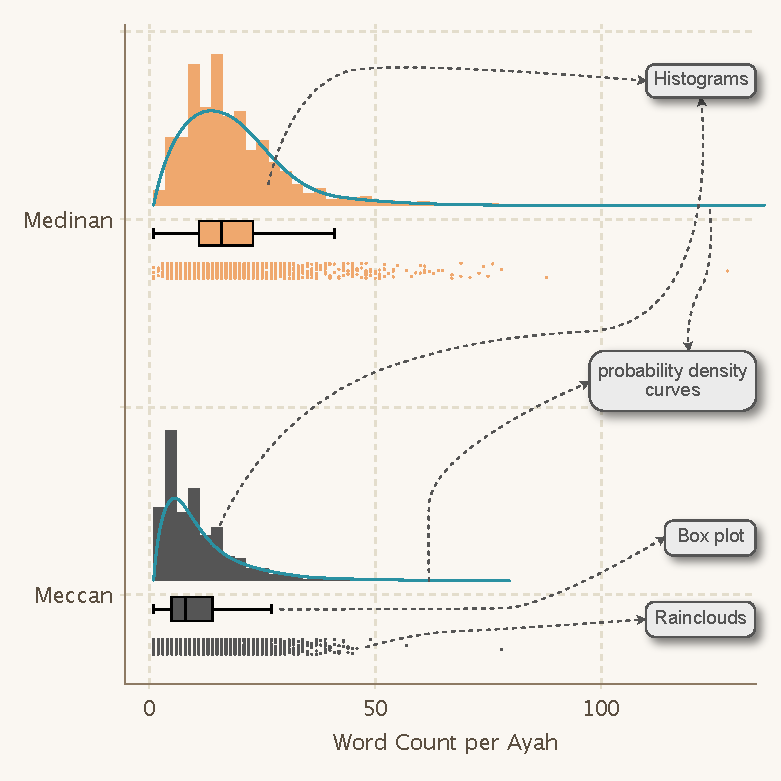
\includegraphics[width=\textwidth]{img/plot3.pdf}
    \caption{Distribution of Meccan and Medinan \arb[trans]{sUwar} \arb{sUwar}}
    \label{fig:result_ayah_word_count_aggregated}
\end{figure}

The main idea of understanding the behavior of data realized from a random phenomenon is not to say it is impossible to describe or understand it, but rather that despite all the uncertainties, it is \textit{possible} to characterize it with the least error compared to other characterizations. The basic way to perform this data-driven characterization is through \textit{sampling distribution}. This is done through data visualization, particularly \textit{histograms} or \textit{box plots}. Figure~\ref{fig:result_ayah_word_count} is a good example of these visualizations. This figure is part of the results of the paper and will be discussed in detail in Chapter~\ref{ch:results}.

To interpret Figure~\ref{fig:result_ayah_word_count}, the histogram and the box plot show the sampling distribution of the \arb[trans]{'ayaT} \arb{'ayaT} counts. In this figure, it tells the reader that the number of \arb[trans]{'ayaT} \arb{'ayaT} counts for those whose \arb[trans]{'asbAb 'alnuzUl} \arb{'asbAb 'alnuzUl} is Meccan is less than those with Medinan \arb[trans]{'asbAb 'alnuzUl} \arb{'asbAb 'alnuzUl}. This is because the median count, shown as the middle line inside the box in the box plot, is closer to zero for Meccan compared to the median count in Medinan. The \textit{location} and \textit{shape} of the histogram tell the reader where it is \textit{concentrated} in terms of the count of \arb[trans]{'ayaT} \arb{'ayaT}, and how \textit{varied} these counts are, respectively. The \textit{rainclouds} in the figure are simply another way of showing the distributions of the data, but this time plotting each of the data points (the ``rain droplets'') instead, and hence the ``droplets'' in the rainclouds plot are concentrated where the peak of the histogram is or where the box of the box plot is. Rainclouds is not a common statistical data visualization tool. Readers are encouraged to consult online resources or basic statistics books to understand how to use these data visualization tools (i.e., histograms and box plots).

\section{Morphological Analysis} \label{sec:method_morph_analysis}
Classical Arabic which the Qur'\=an is written on is very rich in morphology. A root word can have several morphologies, in English for example the root word beauty can have the following morphologies: as Noun, \textit{beauties}, \textit{beautician}, and \textit{beautification}; as Adjective, \textit{beautiful}, \textit{beauteous}, \textit{beautyless}, and \textit{beautified}; as Verb, \textit{beautify}, \textit{beautifies}, \textit{beautified}, and \textit{beautifying}; as Adverb, \textit{beautifully}; with Prefixes, \textit{unbeautiful} and \textit{non-beautiful}.

Now for Arabic, the root words are primarily composed of three consonant letters, and then from these letters different combinations of vowels, prefixes, and suffixes which forms the different morphologies. So for the word \arb[trans]{jamAl} \arb{jamAl}, the root word are the following consonant letters \arb[trans]{jml} \arb[novoc]{jml}. The morphologies from this root word are the following: as Noun, \arb[trans]{jamAl} \arb{jamAl} (beauty), \arb[trans]{jamIl} \arb{jamIl} (beauty, grace; also used as Masculine Adjective), \arb[trans]{majmal} \arb{majmal} (totality, sum), \arb[trans]{tajmIl} \arb{tajmIl} (beautification, embellishment), \arb[trans]{mujAmalaT} \arb{mujAmalaT} (courtesy, compliment, flattery),  \arb[trans]{mujammil} \arb{mujammil} (beautician), \arb[trans]{jamAliyyaT} \arb{jamAliyyaT} (aesthetics); As Adjectives,  \arb[trans]{jamIlaT} \arb{jamIlaT} (beautiful, pretty (Feminine)), \arb[trans]{'ajmal} \arb{'ajmal} (more beautiful, prettier (comparative)), \arb[trans]{mujammal} \arb{mujammal} (beautified, adorned), \arb[trans]{mujmal} \arb{mujmal} (summarized, concise); As Verbs, \arb[trans]{jamula} \arb{jamula} (to be beautiful (perfect tense)), \arb[trans]{yajmulu} \arb{yajmulu} (to be beautiful (imperfect tense)), \arb[trans]{jammala} \arb{jammala} (to beautify, embellish (perfect tense)), \arb[trans]{yujammilu} \arb{yujammilu} (to beautify, embellish (imperfect tense)), \arb[trans]{tajammala} \arb{tajammala} (to make oneself beautiful (perfect tense)), \arb[trans]{yatajammalu} \arb{yatajammalu} (to make oneself beautiful (imperfect tense)), \arb[trans]{jAmala} \arb{jAmala} (to compliment, flatter (perfect tense)), \arb[trans]{yujAmilu} \arb{yujAmilu} (to compliment, flatter (imperfect tense)), \arb[trans]{'ajmala} \arb{'ajmala} (to summarize, do something well (perfect tense)), \arb[trans]{yujmilu} \arb{yujmilu} (to summarize, do something well (imperfect tense)); as Active Particles, \arb[trans]{jAmil} \arb{jAmil} (one who is beautiful), \arb[trans]{mujammil} \arb{mujammil} (one who is beautifies), \arb[trans]{mujAmil} \arb{mujAmil} (one who compliments/flatters); as Passive Particles, \arb[trans]{majmUl}\newline \arb{majmUl} (beautified), \arb[trans]{mujammal} \arb{mujammal} (beautified, embellished), \arb[trans]{mujmal} \arb{mujmal} (summarized); and, finally related forms to it, \arb[trans]{jumlaT} \arb{jumlaT} (sentence, totality), \arb[trans]{'ijmAlI} \arb{'ijmAlI} (total, overall), \arb[trans]{bi-'l-'ijmAlI} \arb{bi-'l-'ijmAlI} (in summary).

From the above examples, it clearly shows the rich morphologies of an Arabic root word. The Qur'\=an with its unique literary style and organizational structure has gain many scholars to understand its underlying structure. Why is it arranged in such way? Is there a hidden pattern that will give insights on how it is structured? For any Muslim believers, such questions may not really be of interests as the answer is not prescriptive of what should a Muslim do and not do. Indeed, it can be considered unnecessary questions to ask. However, just like many great Islamic scholars who have been fascinated by the Qur'\=an, a book containing the literal words of God, it is indeed of great interest to also study how the Creator designed His Book. Indeed, if the premise for this book is that it is the Word of God, wouldn't it be of great interest to study everything in it? To learn its message, its history, its language, and also its structure? Indeed, this is the intention of this section, to study the structure of the Qur'\=an through studying important root words that may help give insights to its structure, and even history of its compilations. To do this, the methodology is straightforward, and that is, to simply find the morphologies of the given root word and understand why it is located in such part of the Qur'\=an, and what does it talks about, meaning the themes of the \arb[trans]{'AyAt} \arb{'AyAt} containing it. The methodology for getting the themes is discussed in the next section.
\section{Thematic Analysis}\label{sec:method_thematic_analysis}
One of the necessary thing to do when it comes to studying the content of group of \arb[trans]{'AyAt} \arb{'AyAt} is to summarize it. Most of the time this is done manually, by reading through the \arb[trans]{'AyAt} \arb{'AyAt} one-by-one, which can take a significant amount of time for number of \arb[trans]{'AyAt} \arb{'AyAt}. Although, such approach if indeed done with more time to reviewing will yield very accurate summaries. This paper, however, will also explore the use of Statistical and Machine Learning techniques to summarizing texts. It is a technique meant to automate the summarization of large number of texts, for example, for 100,000 texts and more. The idea is not to have a very precise summary of topics or themes, but a high-level view of what the texts want to convey. These techniques are especially popular in companies whose interests is on understanding the sentiments of their customers, and understanding the themes of their comments regarding their products, for example. So that, these companies can do interventions on those key themes to improve their service or products.

For this paper, these techniques are also used to get a high-level view of what the \arb[trans]{'AyAt} \arb{'AyAt} want to convey. There are three main techniques to do these in Statistics and Machine Learning, and these are Latent Dirichlet Allocation (LDA), Clustering Topics using Bidirectional Encoder Representation from Transformers (BERT) model, and Generative Pre-trained Transformer (GPT). The first one is the classic approach to topic or thematic modeling. In particular, it was built on the idea that \textit{documents} are mixtures of \textit{topics}, that is, each document contains words from multiple topics in different proportions; and then, topics are distributions over \textit{words}, that is, each topic is represented as a probability distribution over the entire vocabulary, where some words have higher probability than others. Further, LDA assumes documents were created through a specific statistical process: choose a topic mixture for the document, then for each word position, select a topic from this mixture; and then draw a word from that topic's word distribution.

The next technique is the Clustering Topics using Bidirectional Encoder Representation from Transformers (BERT) model, the idea of this is based on the fact that the first step to any text computation, including thematic analysis, requires translation of the texts into its numerical representation. The LDA approach above does this using Term Frequency-Inverse Document Frequency (TF-IDF) technique. However, TF-IDF is a classic approach for embedding texts, and is recent advances in Artificial Intelligence (AI) gave birth into other embedding techniques for numerical representation of a given texts. One of those advances is the BERT model developed by Google researchers. This AI model was trained on a huge corpus, and is able to produce a numerical representation of a given texts with better accuracy compared to the TF-IDF approach. Now, there are many BERT models that have been further fine-tuned to specific problems. So, for Classical Arabic, a model called CL-AraBERT was developed by \citeA{MALHAS2022103068}. This model can be used to represent the Qur'\=an's texts numerically, so that succeeding computational analysis can be done in it, such as the clustering techniques. The clustering technique for BERT models was popularized as BERTopic by \citeA{grootendorst2022bertopic}.

The third technique for topic modeling is through the use of GPT models, these are the models that are used by OpenAI, which is the ChatGPT. Similar to BERT model, it was trained on huge corpus, but it's training was done on sequentially predicting the next best word with great accuracy. Among the three techniques, this is the easiest one to use since there are many free platforms that use this. As such, this paper will use this technique for summarization with random sampling validation from the author to check its summary. In particular, the GPT model that will be used for thematic analysis is the GPT-4o model. 

\section{Rhythmic Analysis}\label{sec:method_rhythmic_analysis}
One of the unique features of the Qur'\=an is its rhythm, it rhymes from the first \arb[trans]{'ayaT} \arb{'ayaT} to the last. Yet it is not a poem where it introduces complex words or forms to prioritize rhythm, but it is also not a prose where it focuses message instead of style, rather it has both. It conveys direct message from God, while doing this with a rhythmic style. An example of this is the first \arb[trans]{sUraT} \arb{sUraT} of the Qur'\=an shown in Table \ref{tbl:surah_alfatihah}. A quick search in the web with search string, "recitation of surah al-fatihah," will give video results of the recitation of the said \arb[trans]{sUraT} \arb{sUraT}, which will help appreciate the rhythm for those who can't read Arabic. In this table, notice the last recited syllable highlighted in red. All of them has a vowel "i" for the rest of the \arb[trans]{'ayaT} \arb{'ayaT}, which help with the rhythm. Now looking at the English translation, which is based on M.A.S. Abdel Haleem's Qur'\=an translation, one can see the straight and clear message this \arb[trans]{sUraT} \arb{sUraT} wants to convey, and is conveyed in rhythmic style. 

\begin{table}[!t]
    \caption{The verses or \arb[trans]{'AyAt} \arb{'AyAt} of \arb[trans]{sUraTu 'l-fAti.haT} \arb{sUraTu 'l-fAti.haT}}
    \begin{tabularx}{\textwidth}{cXr}
        \toprule
        \textbf{No.}&\textbf{Transliteration \& }&\textbf{Verses} or \arb[trans]{'AyAt} \arb{'AyAt}\\
        &\textbf{Translation}&\\
        \midrule
        
        1&\arb[trans]{bismi 'l-lahi 'l-ra.hma_ani 'l-ra\arbcolor[red]{hIm"}\arbcolor[gray]{.i}}&
        \multirow{2}{*}{\arb[fullvoc]{bismi 'l-lahi 'l-ra.hma--_ani 'l-ra\arbcolor[red]{hIm"}\arbcolor[gray]{.i}}}\\[0.1cm]
        &In the name of God, the Lord of Mercy, the Giver of Mercy!&\\[1cm]

        2&\arb[trans]{'l.hamdu lillahi rabbi 'l`Ala\arbcolor[red]{mIn"}\arbcolor[gray]{.a}};&
        \multirow{2}{*}{\arb[fullvoc]{'l-.hamdu lillahi rabbi 'l-`Ala\arbcolor[red]{mIn"}\arbcolor[gray]{.a}}}\\[0.1cm]
        &Praise belongs to God, Lord of the Worlds&\\[1cm]

        3&\arb[trans]{'l-ra.hma_ani 'l-ra\arbcolor[red]{hIm"}\arbcolor[gray]{.i}}&
        \multirow{2}{*}{\arb[fullvoc]{'l-ra.hma--_ani 'l-ra\arbcolor[red]{hIm"}\arbcolor[gray]{.i}}}\\[0.1cm]
        &the Lord of Mercy, the Giver of Mercy&\\[1cm]
        
        4&\arb[trans]{ma--_aliki yawmi 'l-\arbcolor[red]{dIn"}\arbcolor[gray]{.i}}&
        \multirow{2}{*}{\arb[fullvoc]{ma--_aliki yawmi 'l-\arbcolor[red]{dIn"}\arbcolor[gray]{.i}}}\\[0.1cm]
        &Master of the Day of Judgement&\\[1cm]

        5&\arb[trans]{'iyyAka na`budu wa-'iyyaka nasta\arbcolor[red]{`In"}\arbcolor[gray]{.u}}&
        \multirow{2}{*}{\arb[fullvoc]{'iyyAka na`budu wa-'iyyaka nasta\arbcolor[red]{`In"}\arbcolor[gray]{.u}}}\\[0.1cm]
        &It is You we worship; it is You we ask for help&\\[1cm]

        6&\arb[trans]{'ihdinA 'l-.sirA.ta 'l-musta\arbcolor[red]{qIm"}\arbcolor[gray]{.a}}&
        \multirow{2}{*}{\arb[fullvoc]{'ihdinA 'l-.sirA.ta 'l-musta\arbcolor[red]{qIm"}\arbcolor[gray]{.a}}}\\[0.1cm]
        &Guide us to the straight path:&\\[0.6cm]

        7&\arb[trans]{.sirA.ta 'lla_dIna 'an`amta `alayhim .gayri 'l-ma.g.dUbi `alayhim wa-lA 'l-.da'Al\arbcolor[red]{lIn"}\arbcolor[gray]{.a}}&
        \multirow{2}{*}{\arb[fullvoc]{.sirA.ta 'lla_dIna 'an`amta `alayhim .gayri 'l-ma.g.dUbi `alayhim wa-lA 'l-.da'A\arbcolor[red]{lIn"}\arbcolor[gray]{.a}}}\\[0.1cm]
        &the path of those You have blessed, those who incur no anger and who have not gone astray&\\
        \bottomrule
    \end{tabularx}
    \label{tbl:surah_alfatihah}
\end{table}

To study this rhythmic feature, the tools from the Theory of Rhythm \cite{schillinger1946schillinger} by Joseph Schillinger is used. In particular, the said theory aims to formalize mathematically how rhythm can be studied. Different graphs will be used for this study, including the line chart, heatmap, and the \textit{rhythm graph} intoduced by Joseph Schillinger. This paper will use visual inspection from these charts to study the patterns of the rhythms.

\section{Concentrism Structural Analysis}\label{sec:method_genetic_algorithm}
Another structure of the Qur'\=an that was observed recently is the \textit{concentric} or \textit{ring} structure, studied extensively by Raymond Farrin in his book, \textit{Structure and Qur'anic Interpretation: A Study of Symmetry and Coherence in Islam's Holy Text}. This structure suggests that the Qur'\=an follows a circular pattern, where its parts relate to its other in circular orientation. To understand this at a high level, suppose the whole Qur'\=an is divided into seven parts namely: $A-B-C-D-A^{*}-B^{*}-C^{*}$ in arranged in ascending fashion, that is, from first part of the Qur'\=an to the last parts of it. The \textit{concentric} pattern suggests that, $A$ is related to $A^{*}$ in terms of topics, $B$ is related to $B^{*}$, $C$ is related to $C^{*}$, and $D$ is the midpoint where the content of it is not related to any of the parts, so it serves as the center. Corrollary to this, is the \textit{chiasmus}, which is a specific kind of \textit{concentric} structure where the order of ideas or topics is reversed in the second half of the structure. An example of this is, $A-B-B^{*}-A^{*}$.


\section{Programming Language Setup}\label{sec:method_code_setup}
This section discusses the programming language used in this paper. As mentioned in Chapter \ref{ch:introduction}, programming languages are languages that computers can understand. Therefore, these programming languages help us create instructions for computers. Among the available programming languages, the Julia programming language will be used in this study. See the discussion in Chapter \ref{ch:introduction} to understand the justification. Furthermore, in terms of the libraries used, QuranTree.jl\footnote{\url{https://github.com/alstat/QuranTree.jl}} by \citeA{asaad2021qurantree} will be used as the main library for interfacing with the digitized Qur'\=an text; Yunir.jl\footnote{\url{https://github.com/alstat/Yunir.jl}} by \citeA{al_ahmadgaid_b_asaad_yunir} will be used for text analytics; and Kitab.jl\footnote{\url{https://github.com/alstat/Kitab.jl}} by \citeA{al_ahmadgaid_b_asaad_kitab} will be used for interfacing with other Islamicate texts from \mbox{OpenITI}\footnote{\url{https://openiti.org/}}. Finally, all of the code for this paper is stored in a Github repository below:

\begin{center}
    \url{https://github.com/alstat/ma-thesis-codes}
\end{center}